% !TeX root = cluster.tex
\documentclass[paper.tex]{subfiles}

\begin{document}
	\section{Determining the Aggregation Function $A$}
	
	At first glance, the ranking of the variables $\V$ seems entirely subjective. It's not hard to buy that this aggregation function $A$ depends on the given variables, but the manner in which each variable ``positively impacts student performance'' is very dependent on what it actually \emph{means}. Unfortunately for us, the semantics of the data depend on world knowledge tied into the description, and there's no intrinsic reason to prefer any given variables over any other.
	
	Nonetheless, we might be able to exploit internal consistencies in the data to absolve ourselves of needing to manually assign ``goodness'' values to every variable. The idea is as follows: even without knowing anything about what variables do, we might be able to group them by how similar they are -- how often they `stand or fall together'. 
	
	For a given random variable $X : \mathcal{X} = \{x_i\} \to \mathbb{R}$, we have the usual definition of its associated entropy:
	\begin{equation}
		H(X) = - \sum_{x_i \in \mathcal{X}} {P(x_i) \log_2 (P(x_i))},
	\end{equation}
	
	\subsection{Clustering}
	Clustering, too seems to be an impossible problem, so we 
	
	\subsection{Cluster Separation}
	
	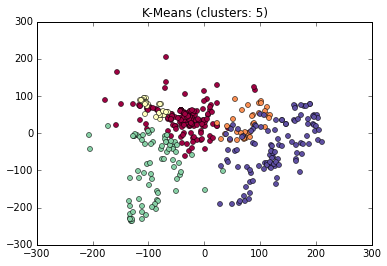
\includegraphics[width=0.5\linewidth]{images/clusters_km_5.png}
	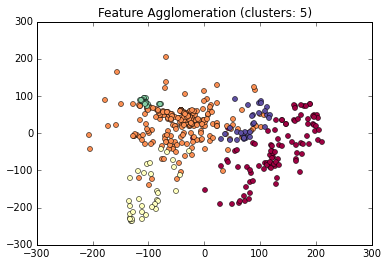
\includegraphics[width=0.5\linewidth]{images/clusters_fa_5.png}
		
	\subsection{Models to Assign Weights}
	
\end{document}